\chapter{Introduction}

The adaptive solar fa\c{c}ade project explores novel integration of photovoltaics technology into building fa\c{c}ades combined with occupant centered control.[1] The aim of the research is to develop architectural systems that are energetically productive, but also respond to the desires of building occupants thereby providing improved comfort.\\
Multiple prototypes where built. The prototype in Figure~\ref{prototype} is characterized by square and triangular solar panels controlled by two servomotors. \\
At this point one question arises: which orientation control lawis required to automate the solar panels?\\
Since the orientation of the solar panels affects both the electricity production and the energy required for the room behind, its control law will derive from multi-objective optimization.\\
This project aims to find the module orientation able to save or even produce the maximal amount of energy.
The energy saving potential is given by the shading effects of the adaptive solar facade, the electricity production instead is generated from the photovoltaics cells. \\
Another goal of this project is to visualize and compare the results obtained by minimizing the heating, cooling and electricity consumption of the building or maximizing the electricity production of the photovoltaics cells.
The only way to obtain a valid result in reasonable period of time is to simulate a portion of the facade. We have chosen to simulate a single room equipped with fifty-four panels because a complete fa\c{c}ade model would require too much computational effort.
This report describes the simulation software used for the simulations as well as the modality in which has been used and the obtained results.\\

\begin{figure}[h]
 \centering
 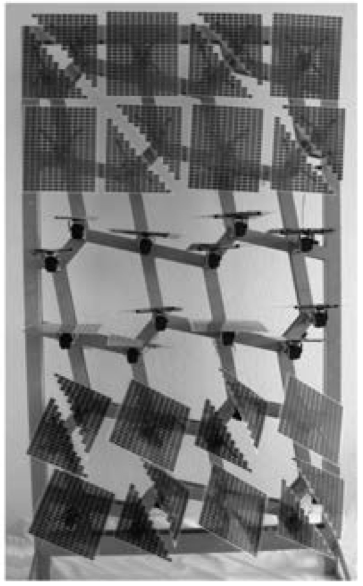
\includegraphics[width=100mm]{graphic/prototype.png}
 \caption{Full scale prototyp for the shading of one window [2]}
 \label{prototype}
\end{figure}